% chapter11.tex - 施瓦西解与黑洞
\chapter{施瓦西解与黑洞 (Schwarzschild Solution and Black Holes)}
\label{chap:schwarzschild}

施瓦西解是爱因斯坦场方程的第一个精确解，由 Karl Schwarzschild 于 1916 年在战场前线（第一次世界大战）推导出来——仅在场方程发表后不到一个月。它描述了球对称、不带电、非旋转的引力源外部的时空几何，并预言了黑洞的存在。本章详细讨论施瓦西度规的性质、测地线运动、黑洞的全局结构、推广解（带电和旋转黑洞）以及黑洞热力学的基本定律。本章是进入广义相对论天体物理应用的基石。

\section{球对称度规与 Birkhoff 定理}
\label{sec:sph_sym}

\subsection{球对称的一般度规形式}

具有球对称性的时空的度规可以在角坐标为通常球坐标 $(\theta,\phi)$ 的情况下写为最一般形式。球对称意味着度规在 $SO(3)$ 旋转群作用下不变，这强烈约束了度规的形式。

\begin{definition}[球对称度规的一般形式]
在球坐标 $(t,r,\theta,\phi)$ 中，最一般的球对称度规可以写为：
\begin{equation}
    \dd s^2 = -A(t,r) \, \dd t^2 + B(t,r) \, \dd r^2 + 2 C(t,r) \, \dd t \dd r + D(t,r) \, r^2 (\dd\theta^2 + \sin^2\theta \, \dd\phi^2),
    \label{eq:gen_sph}
\end{equation}
其中 $A,B,C,D$ 是 $t$ 和 $r$ 的任意函数。通过适当的坐标变换 $t \to t'(t,r)$ 和 $r \to r'(t,r)$，可以消去交叉项 $C(t,r)$ 并设 $D(t,r)=1$（通过重新定义径向坐标）。
\end{definition}

\begin{theorem}[Birkhoff 定理]
\label{thm:birkhoff}
爱因斯坦真空场方程（$T_{\mu\nu}=0$）的球对称解必然是\textbf{静态的}，且由施瓦西度规唯一描述（至多差一个坐标变换）。换言之，球对称的真空引力场：\begin{enumerate}
    \item 必然是静态的——度规系数不依赖于 $t$，即 $\partial_t g_{\mu\nu}=0$；
    \item 必然由单参数质量 $M$ 确定；
    \item 与源（恒星）的内部动力学（如脉动）无关——只要它是球对称的。
\end{enumerate}
\end{theorem}

\begin{note}[Birkhoff 定理的物理意义]
Birkhoff 定理是广义相对论中的一个非平凡结果。在牛顿引力中，球对称质量分布的外部引力场是静态的（与时间无关）——但这是牛顿理论的一个\textbf{假设}，而非定理。在广义相对论中，Birkhoff 定理\textbf{证明}了这个性质：球对称的脉动恒星不会产生引力波（因为度规是静态的，没有时变的四极矩）。这与电磁学形成对比：球对称的振荡电荷\textbf{不能}辐射电磁波（球对称性保证了没有偶极辐射，但可以有单极辐射吗？不，电荷守恒禁止了单极辐射），但引力波需要时变的四极矩（或更高极矩）——Birkhoff 定理的推论正是：球对称系统根本不能辐射引力波 \cite{Wald1984,Carroll1997}。
\end{note}

\subsection{从球对称到施瓦西解的推导概要}

从最一般的球对称度规（\ref{eq:gen_sph}）出发，通过坐标变换消去 $\dd t\dd r$ 交叉项并归一化角向部分，得到：
\begin{equation}
    \dd s^2 = -e^{2\alpha(t,r)} \dd t^2 + e^{2\beta(t,r)} \dd r^2 + r^2 (\dd\theta^2 + \sin^2\theta \, \dd\phi^2).
\end{equation}
计算 Christoffel 符号和 Ricci 张量。真空场方程 $R_{\mu\nu}=0$ 给出：
\begin{align}
    R_{tt} &= e^{2(\alpha-\beta)}\left[\alpha'' + (\alpha')^2 - \alpha'\beta' + \frac{2}{r}\alpha'\right] - \ddot\beta - \dot\beta(\dot\beta-\dot\alpha) = 0, \\
    R_{rr} &= -\left[\alpha'' + (\alpha')^2 - \alpha'\beta' - \frac{2}{r}\beta'\right] + e^{2(\beta-\alpha)}\left[\ddot\beta + \dot\beta(\dot\beta-\dot\alpha)\right] = 0, \\
    R_{tr} &= \frac{2}{r}\dot\beta = 0, \\
    R_{\theta\theta} &= e^{-2\beta}\left[r(\beta'-\alpha')-1\right] + 1 = 0.
\end{align}
由 $R_{tr}=0$ 得 $\dot\beta=0$，即 $\beta=\beta(r)$。然后 $R_{tt}$ 和 $R_{rr}$ 组合可得 $\dot\alpha=0$，故 $\alpha=\alpha(r)$。最后 $R_{\theta\theta}=0$ 结合径向方程给出：
\begin{equation}
    \alpha(r) + \beta(r) = \text{常数} \;\Longrightarrow\; e^{2\alpha} = e^{-2\beta} = 1 - \frac{r_s}{r},
\end{equation}
其中 $r_s$ 是积分常数，通过牛顿极限（$r\to\infty$ 时 $g_{00} \approx -(1 + 2\Phi)$，$\Phi = -GM/r$）确定为 $r_s = 2GM/c^2$。

\section{施瓦西度规}
\label{sec:schwarz_metric}

\begin{definition}[施瓦西度规 —— 标准形式]
在 Schwarzschild 坐标 $(t, r, \theta, \phi)$ 中，质量为 $M$ 的球对称天体外部（真空区域）的时空度规为：
\begin{equation}
    \boxed{\dd s^2 = -\left(1 - \frac{r_s}{r}\right) c^2 \dd t^2 + \left(1 - \frac{r_s}{r}\right)^{-1} \dd r^2 + r^2 (\dd\theta^2 + \sin^2\theta \, \dd\phi^2)},
    \label{eq:schwarz_metric}
\end{equation}
其中 $r_s \equiv 2GM/c^2$ 是\textbf{施瓦西半径 (Schwarzschild radius)}。在自然单位制（$G=c=1$）中，$r_s = 2M$，度规简化为：
\begin{equation}
    \dd s^2 = -\left(1 - \frac{2M}{r}\right) \dd t^2 + \left(1 - \frac{2M}{r}\right)^{-1} \dd r^2 + r^2 \dd\Omega^2,
    \label{eq:schwarz_geom}
\end{equation}
其中 $\dd\Omega^2 \equiv \dd\theta^2 + \sin^2\theta\,\dd\phi^2$ 是单位球面的度规。
\end{definition}

\begin{note}[坐标的有效范围]
施瓦西坐标 $(t,r,\theta,\phi)$ 在以下区域有效：
\begin{itemize}
    \item $r > r_s$（外部区域）：度规是静态的，$t$ 是类时坐标，$r$ 是类空坐标；
    \item $0 < r < r_s$（内部区域）：度规仍然是有效的真空解，但 $t$ 变为类空、$r$ 变为类时——意味着坐标具有不同的物理解释；
    \item $r = r_s$：度规（在 Schwarzschild 坐标中）表现出发散——但这只是坐标奇点，不是曲率奇点。我们将在第 \ref{sec:horizon} 节讨论；
    \item $r = 0$：真正的曲率奇点，Kretschmann 标量 $R^{\mu\nu\rho\sigma}R_{\mu\nu\rho\sigma} = 48M^2/r^6 \to \infty$。
\end{itemize}
\end{note}

\section{施瓦西几何的性质}
\label{sec:geom_prop}

\subsection{Killing 矢量场}

施瓦西时空具有四个线性独立的 Killing 矢量场，反映了其对称性。

\begin{definition}[Killing 方程与守恒量]
Killing 矢量场 $\xi^\mu$ 满足 Killing 方程 $\nabla_\mu \xi_\nu + \nabla_\nu \xi_\mu = 0$。对于测地线 $x^\mu(\lambda)$（$\lambda$ 为仿射参数），沿测地线的量 $\xi_\mu \dot x^\mu$ 是守恒的：
\begin{equation}
    \frac{\dd}{\dd\lambda}(\xi_\mu \dot x^\mu) = 0.
\end{equation}
\end{definition}

\subsection{施瓦西时空的 Killing 矢量}

\begin{itemize}
    \item \textbf{时间平移对称性}：度规不依赖于 $t$，对应的 Killing 矢量为 $\xi_{(t)} = \partial_t = (1,0,0,0)$。这给出\textbf{每单位质量的守恒能量}：
    \begin{equation}
        E \equiv -\xi_{(t)\mu} \dot x^\mu = \left(1 - \frac{2M}{r}\right) \dot t = \text{常数}.
        \label{eq:E_conserved}
    \end{equation}
    
    \item \textbf{旋转对称性}：度规在 $SO(3)$ 下不变，对应三个 Killing 矢量场：
    \begin{align}
        \xi_{(x)} &= -\sin\phi\,\partial_\theta - \cot\theta\cos\phi\,\partial_\phi, \\
        \xi_{(y)} &= \cos\phi\,\partial_\theta - \cot\theta\sin\phi\,\partial_\phi, \\
        \xi_{(z)} &= \partial_\phi.
    \end{align}
    由于球对称性，我们可以选择轨道平面为赤道面 $\theta = \pi/2$。此时 $\xi_{(z)} = \partial_\phi$ 给出\textbf{每单位质量的守恒角动量}：
    \begin{equation}
        L \equiv \xi_{(\phi)\mu} \dot x^\mu = r^2 \dot\phi = \text{常数}.
        \label{eq:L_conserved}
    \end{equation}
\end{itemize}

\subsection{静态性与稳态性}

\begin{definition}[静态时空]
如果时空既具有类时 Killing 矢量场（稳态性），又满足该 Killing 矢量场与超曲面正交（无旋转），则称为\textbf{静态时空 (static spacetime)}。施瓦西时空是静态的：$\xi_{(t)} = \partial_t$ 是类时 Killing 矢量（在 $r>2M$），且与 $t=\text{常数}$ 超曲面正交。
\end{definition}

\section{测地线与轨道}
\label{sec:orbits}

\subsection{测地线方程与有效势}

利用守恒量 $E$ 和 $L$，类时测地线（大质量粒子）的运动可以简化为一维有效势问题。

从四速归一化条件 $g_{\mu\nu}\dot x^\mu\dot x^\nu = -1$（对类时测地线，取 $\tau$ 为本征时），在赤道面 $\theta=\pi/2$ 上代入度规（\ref{eq:schwarz_geom}）：
\begin{equation}
    -\left(1-\frac{2M}{r}\right)\dot t^2 + \left(1-\frac{2M}{r}\right)^{-1}\dot r^2 + r^2\dot\phi^2 = -1.
\end{equation}
利用守恒量 $E = (1-2M/r)\dot t$ 和 $L = r^2\dot\phi$，整理得：
\begin{equation}
    \boxed{\frac{1}{2}\dot r^2 + V_{\text{eff}}(r) = \frac{1}{2}(E^2 - 1)},
    \label{eq:eff_potential}
\end{equation}
其中\textbf{有效势} $V_{\text{eff}}(r)$ 定义为：
\begin{equation}
    \boxed{V_{\text{eff}}(r) = -\frac{M}{r} + \frac{L^2}{2r^2} - \frac{ML^2}{r^3}}.
    \label{eq:Veff}
\end{equation}

\begin{note}[有效势各项的物理意义]
$V_{\text{eff}}(r)$ 中的三项分别对应：
\begin{enumerate}
    \item $-M/r$：牛顿引力势（$c=1$ 单位制）；
    \item $L^2/(2r^2)$：离心势垒——与牛顿力学相同；
    \item $-ML^2/r^3$：\textbf{广义相对论修正项}——以 $1/r^3$ 衰减，在小 $r$ 处主导，导致势在 $r\to 0$ 时趋于 $-\infty$，这是黑洞捕获的本质原因。
\end{enumerate}
\end{note}

\begin{figure}[htbp]
\centering
\begin{tikzpicture}[scale=1.6, >=stealth]
    % 坐标轴
    \draw[->] (0,-1.8) -- (0,1.0) node[above] {$V_{\text{eff}}(r)$};
    \draw[->] (0,0) -- (8.5,0) node[right] {$r/M$};
    
    % 不同L/M值的有效势曲线
    % L/M = 4.5 (最低的那条，有最深的势阱)
    \draw[domain=2.1:8, smooth, variable=\x, blue, thick] 
        plot ({\x}, {-1/\x + 4.5*4.5/(2*\x*\x) - 4.5*4.5/(\x*\x*\x) - 0.25});
        
    % L/M = 4.0
    \draw[domain=2.1:8, smooth, variable=\x, red, thick] 
        plot ({\x}, {-1/\x + 4.0*4.0/(2*\x*\x) - 4.0*4.0/(\x*\x*\x)});
        
    % L/M = 2\sqrt{3} ≈ 3.464 (ISCO boundary)
    \draw[domain=2.1:8, smooth, variable=\x, green!60!black, thick] 
        plot ({\x}, {-1/\x + 3.464*3.464/(2*\x*\x) - 3.464*3.464/(\x*\x*\x) + 0.08});
        
    % L/M = 2.5 (no stable circular orbit)
    \draw[domain=2.1:8, smooth, variable=\x, orange, thick] 
        plot ({\x}, {-1/\x + 2.5*2.5/(2*\x*\x) - 2.5*2.5/(\x*\x*\x) + 0.18});

    % ISCO标记
    \draw[dashed, gray] (6, -0.5) -- (6, 0.7);
    \node[below] at (6, -0.5) {$r=6M$ (ISCO)};
    
    % 光子球标记
    \draw[dashed, gray] (3, -1.0) -- (3, 0.9);
    \node[below] at (3, -0.5) {$r=3M$ (光子球)};
    
    % Schwarzschild 半径
    \draw[dashed, gray] (2, -1.8) -- (2, 1.0);
    \node[below] at (2, -1.0) {$r=2M$};
    
    % 图例
    \node[blue, anchor=west] at (7.0, 0.65) {$L=4.5M$};
    \node[red, anchor=west] at (7.0, 0.45) {$L=4.0M$};
    \node[green!60!black, anchor=west] at (7.0, 0.25) {$L=2\sqrt{3}M$};
    \node[orange, anchor=west] at (7.0, 0.05) {$L=2.5M$};
    
    % 牛顿离心势对比（虚线）
    \draw[domain=2.1:8, smooth, variable=\x, dashed, gray] 
        plot ({\x}, {-1/\x + 4.0*4.0/(2*\x*\x)});
    \node[gray, anchor=west] at (7.0, -0.15) {牛顿 (L=4M)};
\end{tikzpicture}
\caption{施瓦西时空大质量粒子的有效势 $V_{\text{eff}}(r)$ 与径向坐标 $r/M$ 的关系，展示了不同角动量 $L$ 下的曲线。注意广义相对论修正项 $-ML^2/r^3$ 导致 $r\to 0$ 时 $V_{\text{eff}}\to -\infty$，而牛顿有效势（灰色虚线）在 $r\to 0$ 时趋于 $+\infty$（离心势垒主导）。$r=2M$ 是视界，$r=3M$ 是光子球（不稳圆轨道），$r=6M$ 是最内稳定圆轨道 (ISCO)。}
\label{fig:Veff}
\end{figure}

\subsection{圆轨道与 ISCO}

圆轨道满足 $\dot r = 0$ 且 $\ddot r = 0$，即 $V_{\text{eff}}'(r) = 0$：
\begin{equation}
    \frac{M}{r^2} - \frac{L^2}{r^3} + \frac{3ML^2}{r^4} = 0 \;\Longrightarrow\; L^2 = \frac{Mr^2}{r-3M}.
\end{equation}
由此，圆轨道角动量 $L$ 和能量 $E$ 分别为：
\begin{equation}
    L^2 = \frac{Mr^2}{r-3M}, \qquad E^2 = \frac{(r-2M)^2}{r(r-3M)}.
\end{equation}

轨道的稳定性由 $V_{\text{eff}}''(r)$ 的符号决定。最内稳定圆轨道（ISCO, Innermost Stable Circular Orbit）对应 $V_{\text{eff}}''(r)=0$：
\begin{equation}
    V_{\text{eff}}''(r) = 0 \;\Longrightarrow\; r = 6M.
    \label{eq:ISCO}
\end{equation}

\begin{theorem}[施瓦西黑洞的 ISCO]
对于施瓦西黑洞，最内稳定圆轨道 (ISCO) 位于：
\begin{equation}
    \boxed{r_{\text{ISCO}} = 6M = 3r_s}.
\end{equation}
在 ISCO 处，粒子的比角动量为 $L = 2\sqrt{3}M$，比能量为 $E = 2\sqrt{2}/3 \approx 0.943$（即束缚能的 $1 - E \approx 5.7\%$ 被引力势能贡献）。
\end{theorem}

\subsection{光子轨道与光子球}

对于类光测地线（光子），四速归一化条件 $g_{\mu\nu}\dot x^\mu\dot x^\nu = 0$ 给出：
\begin{equation}
    \frac{1}{2}\dot r^2 + \frac{L^2}{2r^2}\left(1 - \frac{2M}{r}\right) = \frac{E^2}{2},
\end{equation}
其中 $b \equiv L/E$ 是\textbf{碰撞参数 (impact parameter)}。有效势为：
\begin{equation}
    V_{\text{eff}}^{\text{null}}(r) = \frac{L^2}{2r^2}\left(1 - \frac{2M}{r}\right).
\end{equation}

\begin{theorem}[光子球]
不稳定光子圆轨道位于 $V_{\text{eff}}^{\text{null}\,'}(r) = 0$ 的解：
\begin{equation}
    \boxed{r_{\text{ph}} = 3M = \frac{3}{2}r_s}.
\end{equation}
这是\textbf{光子球 (photon sphere)}——光子可以在 $r=3M$ 处做（不稳定的）圆轨道运动。对应的碰撞参数为 $b_{\text{crit}} = 3\sqrt{3}M$。
\end{theorem}

\begin{note}[光子球与黑洞阴影]
光子球是黑洞阴影的物理根源。远处观察者看到的黑洞“暗影”对应于碰撞参数 $b < b_{\text{crit}}$ 的光子被黑洞捕获，$b > b_{\text{crit}}$ 的光子逃逸到无穷远。事件视界望远镜 (EHT) 拍摄的 M87* 黑洞照片中的“光环”直径约为 $2\sqrt{27}GM/c^2 \approx 5.2\,r_s$ \cite{Misner1973}。
\end{note}

\subsection{近日点进动}

对于束缚椭圆轨道，轨道方程可以通过引入 $u \equiv 1/r$ 并将 $r$-$\phi$ 关系写为微分方程得到。利用守恒量消去 $\dot t$ 和 $\dot\phi$，得到\textbf{轨道微分方程}：
\begin{equation}
    \frac{\dd^2 u}{\dd\phi^2} + u = \frac{M}{L^2} + 3Mu^2.
    \label{eq:orbit_eq}
\end{equation}

\begin{theorem}[水星近日点进动]
对于 $L \gg M$（弱场极限），方程（\ref{eq:orbit_eq}）的近似解为：
\begin{equation}
    u(\phi) \approx \frac{M}{L^2}\left[1 + e\cos\bigl((1-\delta)\phi\bigr)\right], \qquad \delta = \frac{3M^2}{L^2} \approx \frac{3M}{a(1-e^2)},
\end{equation}
其中 $a$ 是半长轴，$e$ 是偏心率。每圈的近日点进动角为：
\begin{equation}
    \boxed{\Delta\phi_{\text{prec}} = 2\pi\delta = \frac{6\pi M}{a(1-e^2)} = \frac{6\pi GM}{a(1-e^2)c^2}}.
\end{equation}
对于水星：$M_\odot \approx 1.477\,\text{km}$，$a \approx 5.79\times10^7\,\text{km}$，$e\approx0.2056$，给出 $\Delta\phi \approx 43''$ / 世纪——这与观测精确吻合，是广义相对论的经典验证之一。
\end{theorem}

\section{事件视界与黑洞}
\label{sec:horizon}

\subsection{施瓦西坐标的奇点性质}

\begin{definition}[坐标奇点与曲率奇点]
$r=2M$ 处的度规发散是\textbf{坐标奇点 (coordinate singularity)}——可以通过坐标变换消除。$r=0$ 处的发散是\textbf{曲率奇点 (curvature singularity)}——Kretschmann 标量 $K \equiv R^{\mu\nu\rho\sigma}R_{\mu\nu\rho\sigma} = 48M^2/r^6$ 在 $r\to 0$ 时发散，表明它是真正的物理奇点。
\end{definition}

\subsection{Eddington–Finkelstein 坐标}

为了跨越 $r=2M$，引入\textbf{乌龟坐标 (tortoise coordinate)} $r^*$：
\begin{equation}
    r^* \equiv r + 2M\ln\left|\frac{r-2M}{2M}\right|, \qquad \dd r^* = \frac{\dd r}{1-2M/r}.
\end{equation}
在 $(t,r^*)$ 坐标中，径向类光测地线简单地满足 $t \pm r^* = \text{常数}$。

定义\textbf{超前 Eddington–Finkelstein 坐标} $v \equiv t + r^*$（用于描述入射光线），度规变为：
\begin{equation}
    \boxed{\dd s^2 = -\left(1 - \frac{2M}{r}\right) \dd v^2 + 2\,\dd v\dd r + r^2 \dd\Omega^2}.
    \label{eq:EF_metric}
\end{equation}
此度规在 $r=2M$ 处\textbf{非奇异}——所有度规分量都是正则的。入射类光测地线（$v=\text{常数}$）可以平滑地穿过 $r=2M$。

\subsection{Kruskal–Szekeres 延拓}

虽然 Eddington–Finkelstein 坐标消除了 $r=2M$ 处的奇点，但它只覆盖了部分时空。\textbf{Kruskal–Szekeres 坐标}给出了施瓦西时空的\textbf{最大解析延拓}。

\begin{definition}[Kruskal–Szekeres 坐标]
定义新坐标 $(T,X,\theta,\phi)$：
\begin{equation}
    T = \sqrt{\frac{r}{2M}-1}\; e^{r/4M} \sinh\!\left(\frac{t}{4M}\right), \qquad
    X = \sqrt{\frac{r}{2M}-1}\; e^{r/4M} \cosh\!\left(\frac{t}{4M}\right), \qquad (r > 2M)
\end{equation}
\begin{equation}
    T = \sqrt{1-\frac{r}{2M}}\; e^{r/4M} \cosh\!\left(\frac{t}{4M}\right), \qquad
    X = \sqrt{1-\frac{r}{2M}}\; e^{r/4M} \sinh\!\left(\frac{t}{4M}\right), \qquad (r < 2M)
\end{equation}
满足 $T^2 - X^2 = \left(1 - \frac{r}{2M}\right)e^{r/2M}$。度规变为：
\begin{equation}
    \boxed{\dd s^2 = \frac{32M^3}{r}\, e^{-r/2M}\,(-\dd T^2 + \dd X^2) + r^2 \dd\Omega^2},
    \label{eq:KS_metric}
\end{equation}
其中 $r$ 由 $T^2 - X^2 = (1-r/2M)e^{r/2M}$ 隐式定义。
\end{definition}

\begin{figure}[htbp]
\centering
\begin{tikzpicture}[scale=2.5, >=stealth]
    % 背景区域划分
    % Region I (我们的宇宙, r > 2M): X > |T|
    \fill[blue!8] (0,0) -- (4.5,4.5) -- (0,4.5) -- cycle;
    \fill[blue!8] (0,0) -- (4.5,-4.5) -- (0,-4.5) -- cycle;
    
    % Region II (黑洞, r < 2M): T > |X|
    \fill[red!10] (0,0) -- (4.5,4.5) -- (-4.5,4.5) -- cycle;
    
    % Region III (白洞, r < 2M): T < -|X|
    \fill[green!10] (0,0) -- (4.5,-4.5) -- (-4.5,-4.5) -- cycle;
    
    % Region IV (平行宇宙, r > 2M): X < -|T|
    \fill[yellow!8] (0,0) -- (-4.5,4.5) -- (-4.5,-4.5) -- cycle;
    
    % 奇点 r=0 (双曲线) — 使用显式坐标以避免 Dimension too large
    \draw[red, very thick] (4.5,0) .. controls (5.5,1.5) and (7.0,3.5) .. (8.2,5.5);
    \draw[red, very thick] (4.5,0) .. controls (5.5,-1.5) and (7.0,-3.5) .. (8.2,-5.5);
    \draw[green!60!black, very thick] (-4.5,0) .. controls (-5.5,1.5) and (-7.0,3.5) .. (-8.2,5.5);
    \draw[green!60!black, very thick] (-4.5,0) .. controls (-5.5,-1.5) and (-7.0,-3.5) .. (-8.2,-5.5);
    
    % 视界 r=2M (对角线)
    \draw[gray, thick, dashed] (-4.5,-4.5) -- (4.5,4.5) node[midway, above left, font=\small] {$r=2M$};
    \draw[gray, thick, dashed] (-4.5,4.5) -- (4.5,-4.5) node[midway, above right, font=\small] {$r=2M$};
    
    % 坐标轴
    \draw[->] (-4.8,0) -- (5.0,0) node[below] {$X$};
    \draw[->] (0,-4.8) -- (0,5.0) node[left] {$T$};
    
    % r=常数曲线 (仅 r < 2 以避免 sqrt 负值)
    \foreach \r in {0.5, 0.8, 1.2, 1.6} {
        \draw[gray!50, thin] plot[domain=-1.8:1.8, smooth, variable=\t]
            ({sqrt((1-\r/2)*exp(\r/2) + \t*\t)}, {\t});
    }
    
    % 标签
    \node[font=\small] at (2.5, 0.8) {I (我们的宇宙)};
    \node[font=\small] at (0.2, 2.8) {II (黑洞)};
    \node[font=\small] at (0.2, -2.8) {III (白洞)};
    \node[font=\small] at (-2.5, 0.8) {IV (平行宇宙)};
    
    \node[red] at (4.6, 2.6) {$r=0$ (未来奇点)};
    \node[green!60!black] at (4.6, -2.2) {$r=0$ (过去奇点)};
    
    % 光锥例子
    \draw[->, blue] (2.0, 0.5) -- (2.5, 0.7);
    \draw[->, blue] (2.0, 0.5) -- (2.5, 0.3);
\end{tikzpicture}
\caption{施瓦西时空的 Kruskal–Szekeres 最大解析延拓。区域 I 是我们的渐近平坦宇宙（$r>2M$），区域 II 是黑洞内部（$r<2M$，任何类时或类光曲线都朝向 $r=0$ 的奇点），区域 III 是白洞内部（所有曲线从 $r=0$ 出来），区域 IV 是另一个渐近平坦宇宙。对角线 $T = \pm X$ 是事件视界 $r=2M$。}
\label{fig:kruskal}
\end{figure}

\subsection{Penrose 图}

Penrose 图通过共形变换将无穷远“拉近”，使整个时空的因果结构一目了然。

\begin{figure}[htbp]
\centering
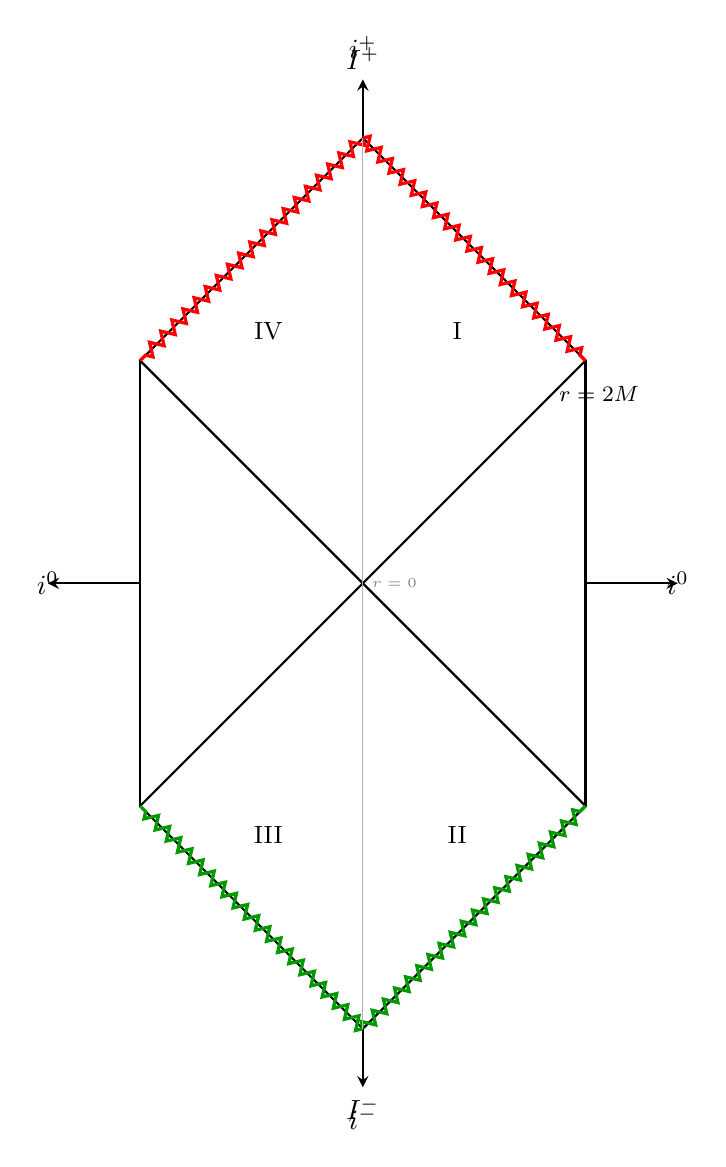
\begin{tikzpicture}[scale=4.0, >=stealth]
    % 钻石形边界
    \draw[thick] (0,0) -- (0.707,0.707) -- (0,1.414) -- (-0.707,0.707) -- cycle;
    \draw[thick] (0,0) -- (-0.707,-0.707) -- (0,-1.414) -- (0.707,-0.707) -- cycle;
    \draw[thick] (-0.707,0.707) -- (-0.707,-0.707);
    \draw[thick] (0.707,0.707) -- (0.707,-0.707);
    
    % 未来类光无穷远 I+
    \draw[thick, ->] (0,1.414) -- (0,1.6) node[above] {$\mathscr{I}^+$};
    % 过去类光无穷远 I-
    \draw[thick, ->] (0,-1.414) -- (0,-1.6) node[below] {$\mathscr{I}^-$};
    % 类空无穷远 i0
    \node at (1.0, 0) {$i^0$};
    \draw[thick, ->] (0.707,0) -- (1.0,0);
    \node at (-1.0, 0) {$i^0$};
    \draw[thick, ->] (-0.707,0) -- (-1.0,0);
    % 未来类时无穷远 i+
    \node at (0, 1.7) {$i^+$};
    % 过去类时无穷远 i-
    \node at (0, -1.7) {$i^-$};
    
    % 标签
    \node[font=\small] at (0.3, 0.8) {I};
    \node[font=\small] at (-0.3, 0.8) {IV};
    \node[font=\small] at (0.3, -0.8) {II};
    \node[font=\small] at (-0.3, -0.8) {III};
    
    % 奇点 (波浪线)
    \draw[red, very thick, decorate, decoration={zigzag, amplitude=0.8mm, segment length=2mm}] 
        (0,1.414) -- (0.707,0.707);
    \draw[red, very thick, decorate, decoration={zigzag, amplitude=0.8mm, segment length=2mm}] 
        (0,1.414) -- (-0.707,0.707);
    
    \draw[green!60!black, very thick, decorate, decoration={zigzag, amplitude=0.8mm, segment length=2mm}] 
        (0,-1.414) -- (0.707,-0.707);
    \draw[green!60!black, very thick, decorate, decoration={zigzag, amplitude=0.8mm, segment length=2mm}] 
        (0,-1.414) -- (-0.707,-0.707);
    
    % r=常数线
    \draw[gray!60, thin] (0,1.414) -- (0,-1.414);
    \node[font=\tiny, gray] at (0.1, 0.0) {$r=0$};
    
    % 视界标注
    \node[font=\footnotesize] at (0.75, 0.6) {$r=2M$};
\end{tikzpicture}
\caption{施瓦西时空的 Penrose 图（共形图）。整个无限时空被压缩到有限区域内，类光测地线以 $45^\circ$ 角传播。区域 I 是我们的宇宙，II 是黑洞，III 是白洞，IV 是另一个宇宙。$\mathscr{I}^\pm$ 是类光无穷远，$i^0$ 是类空无穷远，$i^\pm$ 是类时无穷远。波浪线表示曲率奇点 $r=0$。}
\label{fig:penrose}
\end{figure}

\begin{definition}[事件视界]
\textbf{事件视界 (event horizon)}是类光无穷远 $\mathscr{I}^+$ 的过去边界的边界——即所有不能到达 $\mathscr{I}^+$ 的事件构成的区域的边界。在施瓦西时空中，事件视界是 $r=2M$ 的类光超曲面：任何穿过 $r=2M$ 进入区域 II 的粒子或光线都无法再逃逸到区域 I。
\end{definition}

\section{Reissner–Nordström 与 Kerr 黑洞}
\label{sec:RN_Kerr}

\subsection{Reissner–Nordström 黑洞（带电黑洞）}

爱因斯坦–Maxwell 场方程描述了带电引力源的外度规。

\begin{definition}[Reissner–Nordström 度规]
质量为 $M$、电荷为 $Q$ 的球对称带电黑洞的度规为：
\begin{equation}
    \boxed{\dd s^2 = -\Delta(r)\,\dd t^2 + \Delta(r)^{-1}\,\dd r^2 + r^2\,\dd\Omega^2},
    \label{eq:RN_metric}
\end{equation}
其中 $\Delta(r) \equiv 1 - \frac{2M}{r} + \frac{Q^2}{r^2}$。相应的电磁场为 $F = \frac{Q}{r^2}\,\dd t \wedge \dd r$。
\end{definition}

\begin{theorem}[RN 黑洞的视界结构]
$\Delta(r)=0$ 的根给出视界位置：
\begin{equation}
    r_\pm = M \pm \sqrt{M^2 - Q^2}.
\end{equation}
根据 $Q$ 与 $M$ 的关系，分三种情况：
\begin{itemize}
    \item $|Q| < M$：\textbf{次极端 RN 黑洞}——有两个视界：$r_+$（外视界/事件视界），$r_-$（内视界/Cauchy 视界）；
    \item $|Q| = M$：\textbf{极端 RN 黑洞}——$r_+ = r_- = M$，单一退化视界，表面引力 $\kappa = 0$；
    \item $|Q| > M$：\textbf{裸奇点}——没有视界，奇点 $r=0$ 是裸露的。宇宙监督假设 (Cosmic Censorship) 推测这种情况在物理上不会发生 \cite{Penrose1965}。
\end{itemize}
\end{theorem}

\subsection{Kerr 黑洞（旋转黑洞）}

Roy Kerr 于 1963 年发现了描述旋转黑洞的精确解——这是天体物理中最重要的一类黑洞，因为实际黑洞通常具有角动量。

\begin{definition}[Kerr 度规 —— Boyer–Lindquist 坐标]
在 Boyer–Lindquist 坐标 $(t,r,\theta,\phi)$ 中，质量为 $M$、角动量为 $J = aM$ 的 Kerr 度规为：
\begin{equation}
    \boxed{\dd s^2 = -\left(1-\frac{2Mr}{\Sigma}\right)\dd t^2 - \frac{4aMr\sin^2\theta}{\Sigma}\,\dd t\dd\phi + \frac{\Sigma}{\Delta}\,\dd r^2 + \Sigma\,\dd\theta^2 + \left(r^2+a^2+\frac{2Mra^2\sin^2\theta}{\Sigma}\right)\sin^2\theta\,\dd\phi^2},
    \label{eq:Kerr_metric}
\end{equation}
其中：
\begin{equation}
    \Sigma \equiv r^2 + a^2\cos^2\theta, \qquad \Delta \equiv r^2 - 2Mr + a^2.
\end{equation}
参数 $a \equiv J/M$ 是\textbf{比角动量 (specific angular momentum)}，满足 $0 \leq a \leq M$。
\end{definition}

\begin{theorem}[Kerr 黑洞的视界与能层]
$\Delta = 0$ 给出两个视界：
\begin{equation}
    r_\pm = M \pm \sqrt{M^2 - a^2}.
\end{equation}
$g_{tt}=0$ 给出\textbf{静界 (static limit)}：
\begin{equation}
    r_{\text{sl}}(\theta) = M + \sqrt{M^2 - a^2\cos^2\theta}.
\end{equation}
视界 $r_+$ 与静界之间的区域称为\textbf{能层 (ergosphere)}。在能层内，任何观者必须随黑洞旋转——无法保持静态（相对于无穷远观者静止），但仍可以逃逸到无穷远。
\end{theorem}

\begin{note}[Penrose 过程 —— 从旋转黑洞提取能量]
在能层中，粒子可以分裂为两部分：一部分落入黑洞（负能量轨道），另一部分逃逸到无穷远——带着比原粒子更多的能量。这个过程称为\textbf{Penrose 过程}，理论上可以从旋转黑洞中提取旋转能。可提取的最大能量为 $M - M_{\text{irr}}$，其中不可约质量 $M_{\text{irr}} = \sqrt{\frac{1}{2}(M^2 + \sqrt{M^4 - J^2})}$。极端 Kerr 黑洞（$a=M$）中多达 $29\%$ 的质量能量可以被提取 \cite{Misner1973}。
\end{note}

\subsection{Kerr–Newman 黑洞}

最一般的稳态黑洞解是 Kerr–Newman 度规，包含质量 $M$、电荷 $Q$ 和角动量 $a$：
\begin{equation}
    \Delta = r^2 - 2Mr + a^2 + Q^2, \qquad \Sigma = r^2 + a^2\cos^2\theta.
\end{equation}
视界位于 $\Delta=0$ 的根：$r_\pm = M \pm \sqrt{M^2 - a^2 - Q^2}$。极端条件为 $M^2 = a^2 + Q^2$。

\subsection{无毛定理 (No-hair Theorem)}

\begin{theorem}[黑洞无毛定理]
在四维爱因斯坦–Maxwell 理论中，稳态黑洞由且仅由三个参数完全描述：
\begin{equation}
    \boxed{M\;(\text{质量}),\quad J\;(\text{角动量}),\quad Q\;(\text{电荷})}.
\end{equation}
所有其他信息（如形成黑洞的物质的初始多极矩）在引力坍缩过程中被辐射掉了。黑洞是“最简单”的宏观物体 \cite{Wald1984,Carroll1997}。
\end{theorem}

\section{黑洞热力学}
\label{sec:BH_thermo}

黑洞热力学是 20 世纪理论物理学最深刻的发现之一——它揭示了引力、量子力学和热力学之间的深层联系。

\subsection{黑洞力学四定律}

\begin{theorem}[黑洞力学四定律]
\label{thm:four_laws}
\begin{enumerate}
    \item \textbf{第零定律}：稳态黑洞的\textbf{表面引力 (surface gravity)} $\kappa$ 在视界上处处为常数（类似于热力学第零定律中温度的均匀性）。
    
    \item \textbf{第一定律}：黑洞质量 $M$、面积 $A$、角动量 $J$ 和电荷 $Q$ 满足：
    \begin{equation}
        \boxed{\dd M = \frac{\kappa}{8\pi G}\,\dd A + \Omega_H\,\dd J + \Phi_H\,\dd Q},
        \label{eq:first_law}
    \end{equation}
    其中 $\Omega_H$ 是视界角速度，$\Phi_H$ 是视界电势。这类似于热力学第一定律 $\dd U = T\dd S + \Omega\dd J + \Phi\dd Q$。
    
    \item \textbf{第二定律 (Hawking 面积定理)}：在经典广义相对论中（满足零能量条件），黑洞视界面积永不减少：
    \begin{equation}
        \boxed{\delta A \geq 0}.
        \label{eq:area_theorem}
    \end{equation}
    这类似于热力学第二定律中熵的单调增加。
    
    \item \textbf{第三定律}：不能通过任何有限步骤将黑洞的表面引力 $\kappa$ 降为零（即不能形成极端黑洞）。这类似于热力学第三定律中不能通过有限步骤达到绝对零度。
\end{enumerate}
\end{theorem}

\subsection{Bekenstein–Hawking 熵}

最初，黑洞力学四定律被认为仅是形式上的类比——毕竟，经典黑洞只能吸收、不能辐射，按定义温度应为零。1972 年，Jacob Bekenstein 大胆提出：黑洞面积\textbf{就是}熵（乘以适当常数），黑洞具有真实的\textbf{热力学}性质 \cite{Wald1984}。

\begin{theorem}[Bekenstein–Hawking 熵公式]
黑洞的熵正比于其视界面积：
\begin{equation}
    \boxed{S_{\text{BH}} = \frac{k_B c^3 A}{4G\hbar} = \frac{A}{4G} \quad (\text{Planck 单位: } k_B = \hbar = c = 1)}.
    \label{eq:BH_entropy}
\end{equation}
在 Planck 单位制中（$G = \ell_P^2$），$S = A/(4\ell_P^2)$——即视界的每个 Planck 面积单元承载约 $\frac{1}{4}\ln 2$ 比特的信息。
\end{theorem}

\begin{note}[广义第二定律]
Bekenstein 提出了\textbf{广义第二定律 (Generalized Second Law, GSL)}：黑洞外物质熵 $S_{\text{matter}}$ 与黑洞熵 $S_{\text{BH}}$ 之和永不减少：
\begin{equation}
    \delta(S_{\text{BH}} + S_{\text{matter}}) \geq 0.
\end{equation}
GSL 将热力学第二定律推广到了包含黑洞的系统中。
\end{note}

\subsection{Hawking 辐射}

1974 年，Stephen Hawking 做出了划时代的发现：将量子场论应用于黑洞时空背景，黑洞\textbf{确实会辐射}——而且是以精确的热谱辐射！

\begin{theorem}[Hawking 辐射与黑洞温度]
施瓦西黑洞以温度为 $T_H$ 的黑体谱辐射粒子：
\begin{equation}
    \boxed{T_H = \frac{\hbar c^3}{8\pi G M k_B} = \frac{\hbar \kappa}{2\pi k_B c} \quad (\text{其中 } \kappa = \frac{c^4}{4GM} \text{ 是表面引力})}.
    \label{eq:Hawking_temp}
\end{equation}
在 Planck 单位中：$T_H = 1/(8\pi M)$。对于太阳质量的黑洞，$T_H \sim 6\times10^{-8}\,\text{K}$——远低于宇宙微波背景温度，因此天体物理黑洞是净吸收者。对于微型原初黑洞（$M \sim 10^{15}\,\text{g}$），$T_H \sim 10^{11}\,\text{K}$，会剧烈蒸发 \cite{Hawking1974}。
\end{theorem}

\begin{note}[Hawking 辐射的物理图像]
量子场论在弯曲时空中的真空不稳定性导致粒子对的产生：在视界附近，虚粒子对中的一个可能落入黑洞（携带负能量），另一个逃逸到无穷远（表现为正能量粒子）。净效果是黑洞质量减少——黑洞“蒸发”。这统一了黑洞力学四定律与真实的热力学：$\kappa/(2\pi)$ 就是黑洞的物理温度，$A/(4G)$ 就是黑洞的物理熵。
\end{note}

\subsection{黑洞热力学与全息原理}

Bekenstein–Hawking 熵公式 $S = A/(4G)$ 具有深远的意义：熵（通常被认为是广延量，正比于体积）在这里正比于\textbf{面积}。这暗示了\textbf{全息原理 (Holographic Principle)}——量子引力理论中，一个空间区域内的全部信息可以编码在该区域的边界上。这是 AdS/CFT 对偶和量子引力研究中的核心思想。

\section{算例与验证}
\label{sec:examples}

\subsection{例 1：计算 ISCO 处的轨道角速度}

对于施瓦西黑洞 $r_{\text{ISCO}} = 6M$ 处的圆轨道：
\begin{equation}
    \Omega = \frac{\dd\phi}{\dd t} = \frac{\dot\phi}{\dot t} = \frac{L/r^2}{E/(1-2M/r)}.
\end{equation}
在 $r=6M$ 处，$L=2\sqrt{3}M$，$E=2\sqrt{2}/3$，代入得：
\begin{equation}
    \Omega_{\text{ISCO}} = \frac{1}{6\sqrt{6}M} \approx \frac{0.068}{M}.
\end{equation}
对应的轨道周期为 $T = 2\pi/\Omega \approx 92.3M$。

\subsection{例 2：Eddington–Finkelstein 坐标中验证 $r=2M$ 处度规正则}

在 Eddington–Finkelstein 坐标（\ref{eq:EF_metric}）中，度规分量为：
\begin{equation}
    g_{vv} = -\left(1-\frac{2M}{r}\right), \quad g_{vr}=g_{rv}=1, \quad g_{rr}=0, \quad g_{\theta\theta}=r^2, \quad g_{\phi\phi}=r^2\sin^2\theta.
\end{equation}
在 $r=2M$ 处，$g_{vv}=0$，$g_{vr}=1$，$g_{rr}=0$。行列式：
\begin{equation}
    \det(g_{\mu\nu}) = -r^4\sin^2\theta \neq 0 \quad (\text{在 } r=2M \text{ 处仍非零}).
\end{equation}
所有度规分量都是有限且可逆的——度规在 $r=2M$ 处完全正则。

\subsection{例 3：验证 $r=2M$ 是类光超曲面}

$r=2M$ 超曲面的法矢量为 $n_\mu = \partial_\mu r = (0,1,0,0)$。其模方为：
\begin{equation}
    g^{\mu\nu}n_\mu n_\nu = g^{rr} = 1 - \frac{2M}{r}.
\end{equation}
在 $r=2M$ 处，$g^{rr}=0$——法矢量是\textbf{类光}的（模方为零）。因此 $r=2M$ 是一个\textbf{类光超曲面 (null hypersurface)}，这正是事件视界的定义特征：它是单向膜——粒子只能向 $r$ 减小的方向穿过它。验证：在 Eddington–Finkelstein 坐标中，入射类光测地线 $v=\text{常数}$ 穿过 $r=2M$ 时满足 $\dd r/\dd\lambda < 0$ 对于正向仿射参数永远成立。

\subsection{例 4：计算太阳质量黑洞的 Hawking 温度与蒸发时间}

取 $M = M_\odot \approx 2\times10^{30}\,\text{kg}$。
\begin{align}
    T_H &= \frac{\hbar c^3}{8\pi G M k_B} \approx 6.2\times10^{-8}\,\text{K}, \\
    r_s &= \frac{2GM}{c^2} \approx 3.0\,\text{km}, \\
    A &= 4\pi r_s^2 \approx 1.1\times10^{8}\,\text{m}^2, \\
    S_{\text{BH}} &= \frac{k_B A}{4\ell_P^2} \approx 1.1\times10^{77}\,k_B.
\end{align}
由 Stefan–Boltzmann 定律（近似），蒸发时间尺度为：
\begin{equation}
    \tau_{\text{evap}} \sim \frac{M^3}{3\alpha}, \qquad \alpha \sim 10^{-4} \;\Longrightarrow\; \tau_{\text{evap}} \sim 10^{67}\,\text{年},
\end{equation}
远大于宇宙年龄（$\sim 1.38\times10^{10}$ 年）——天体物理黑洞在当前宇宙中几乎不蒸发。

\subsection{例 5：Kruskal 坐标中的类时 Killing 矢量}

在 Kruskal 坐标中，$\xi_{(t)} = \partial_t$ 变为：
\begin{equation}
    \xi_{(t)} = \frac{1}{4M}\left(X\,\partial_T + T\,\partial_X\right).
\end{equation}
其模方为：
\begin{equation}
    \xi_{(t)}^\mu \xi_{(t)\mu} = -\left(1-\frac{2M}{r}\right) = \frac{2M}{r}\cdot\frac{T^2-X^2}{T^2-X^2} \cdot (\text{因子}).
\end{equation}
在 $r=2M$（$T^2=X^2$）处，$\xi_{(t)}$ 是类光的；在 $r<2M$（$T^2>X^2$）处，$\xi_{(t)}$ 变为类空——在黑洞内部，$t$ 不再是时间坐标，$r$ 才是时间坐标。这完美展示了事件视界作为“时间与空间角色互换”的边界 \cite{Carroll1997}。

\section*{本章小结}

施瓦西解是爱因斯坦场方程最简单却最重要的精确解。Birkhoff 定理确保球对称真空解必然是静态的施瓦西度规。通过分析 Killing 矢量与守恒量 $E$ 和 $L$，测地线问题简化为有效势的一维运动。广义相对论修正项 $-ML^2/r^3$ 导致 ISCO 在 $r=6M$、光子球在 $r=3M$，以及近日点进动 $\Delta\phi = 6\pi M/[a(1-e^2)]$。

坐标奇点 $r=2M$ 可通过 Eddington–Finkelstein 或 Kruskal–Szekeres 坐标消除，揭示 $r=2M$ 是事件视界——一个类光超曲面。Kruskal 最大解析延拓展现了四个区域：两个渐近平坦宇宙、一个黑洞和一个白洞。推广到带电（RN）和旋转（Kerr）黑洞引入了更丰富的视界结构、能层和 Penrose 过程。

黑洞热力学将经典黑洞力学四定律与真实的热力学统一起来。Bekenstein 熵 $S = A/(4G)$ 和 Hawking 温度 $T_H = \kappa/(2\pi)$ 揭示了引力、量子和热力学的深层联系，为全息原理和量子引力研究铺平了道路。黑洞不再仅是“引力监狱”——它们是具有温度、熵的热力学系统，能够通过 Hawking 辐射缓慢蒸发。黑洞物理是 21 世纪理论物理最活跃的前沿领域之一。
